% !TeX root = ../main.tex

\chapter{低本底模组设计}
\label{chap:LowBackgroundModule}

\section{低本底模组V2修改方案}

\subsection{阳极板修改}

连接器的连接器引脚分布如图 \ref{fig:AB_v1_pins}所示,其中边缘引脚(\emph{X1, Y20, X21, Y40, X41, Y60})容易受干扰,需要重新设计。建议改为Hirose连接器!

\begin{figure}[htbp]
	\centering
	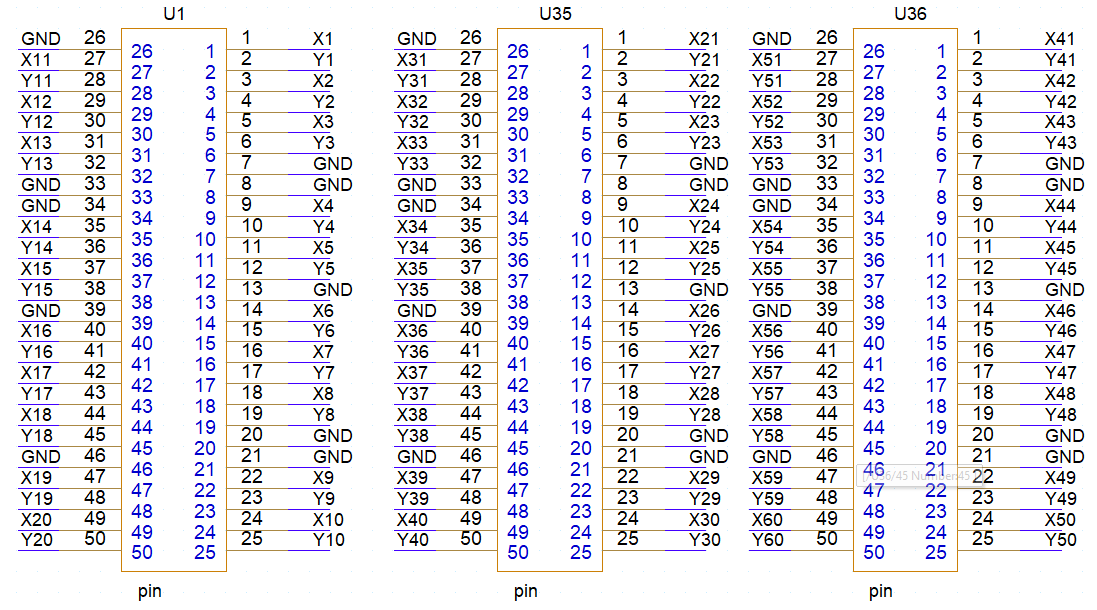
\includegraphics[width=\textwidth]{figures/AB_v1_pins.png}
	\caption{阳极板V1连接器引脚定义}
	\label{fig:AB_v1_pins}
\end{figure}

\subsection{场笼方案}

场笼采用柔性材料 PCB,单层板即可,在横向方向上铺设平行铜皮,全板开窗,铜皮尽可能窄,铜皮间距尽可能小。然后在PCB上均匀镀锗!



